% ОБЯЗАТЕЛЬНО ИМЕННО ТАКОЙ documentclass!
% (Основной кегль = 14pt, поэтому необходим extsizes)
% Формат, разумеется, А4
% article потому что стандарт не подразумевает разделов
% Глава = section, Параграф = subsection
% (понятия "глава" и "параграф" из документа, описывающего диплом)
\documentclass[a4paper,14pt]{extarticle}

% Подключаем главный пакет со всем необходимым
\usepackage{diploma}

\addbibresource{literature.bib} %Import the bibliography file

% Пакеты по желанию (самые распространенные)
% Таблицы
\usepackage{longtable}
\usepackage{makecell}
% Картинки (можно встявлять даже pdf)
\usepackage[pdftex]{graphicx}

\usepackage{amsthm,amssymb, amsmath}
\usepackage{textcomp}

% Подсветка кода (все стили в файле)
\usepackage{color}
\usepackage{listings}
\definecolor{GrayCodeBlock}{RGB}{248,252,255}
\definecolor{BlackText}{RGB}{41,75,102}
\definecolor{RedTypename}{RGB}{182,86,17}
\definecolor{GreenString}{RGB}{96,172,57}
\definecolor{PurpleKeyword}{RGB}{184,84,212}
\definecolor{GrayComment}{RGB}{100,100,100}
\definecolor{GoldDocumentation}{RGB}{180,165,45}

\lstset{
    columns=fullflexible,
    keepspaces=true,
    frame=single,
    framesep=0pt,
    framerule=0pt,
    framexleftmargin=4pt,
    framexrightmargin=4pt,
    framextopmargin=5pt,
    framexbottommargin=3pt,
    xleftmargin=4pt,
    xrightmargin=4pt,
    backgroundcolor=\color{GrayCodeBlock},
    basicstyle=\ttfamily\small\color{BlackText},
    keywordstyle=\color{PurpleKeyword},
    ndkeywordstyle=\color{RedTypename},
    comment=[l][\color{GrayComment}\slshape]{//},
    morecomment=[s][\color{GrayComment}\slshape]{/*}{*/},
    morecomment=[s][\color{RedTypename}]{\#![}{]},
    morecomment=[s][\color{RedTypename}]{\#[}{]},
    stringstyle=\color{GreenString},
    string=[b]"
}

\lstdefinelanguage{rust}
{
    keywords={
        true,false,
        unsafe,async,await,move,
        use,pub,crate,super,self,mod,
        struct,enum,fn,const,static,let,mut,ref,type,impl,dyn,trait,where,as,
        break,continue,if,else,while,for,loop,match,return,yield,in
    },
    ndkeywords={
        bool,u8,u16,u32,u64,u128,i8,i16,i32,i64,i128,char,str,
        Self,Option,Some,None,Result,Ok,Err,String,Box,Vec,Rc,Arc,Cell,RefCell,HashMap,BTreeMap,
        macro_rules
    },
    comment=[l][\color{GrayComment}\slshape]{//}
}


\begin{document}

% Титульник в файле titlepage.tex
\newgeometry{left=30mm, top=20mm, right=15mm, bottom=20mm, nohead, nofoot}
\begin{titlepage}
\begin{center}

Федеральное государственное автономное \\образовательное учреждение высшего образования

\textbf{<<Национальный исследовательский ядерный университет}
\textbf{<<МИФИ>>}

\vspace{35mm}

\textbf{\textit{\large Музыкина Екатерина Андреевна}} \\[8mm]
% Название
\textbf{\large Выпускная квалификационная работа}\\[3mm]
\textbf{\textit{\large Название работы}}

\vspace{20mm}
Уровень образования: магистратура\\
Направление 11.04.04 «Электроника и наноэлектроника»\\
Образовательная программа
«Наноэлектроника, спинтроника и фотоника»\\[25mm]


% Научный руководитель, рецензент
\begin{flushright}
\begin{minipage}[t]{0.5\textwidth}
{Научный руководитель:} \\
к.ф.-м.н., доцент кафедры \\физики конденсированных сред, \\ Сибирмовский Ю.Д.

\vspace{10mm}

{Рецензент:} \\
 \\
\end{minipage}
\end{flushright}

\vfill 

{Москва}
\par{\the\year{} г.}
\end{center}
\end{titlepage}
% Возвращаем настройки geometry обратно (то, что объявлено в преамбуле)
\restoregeometry
% Добавляем 1 к счетчику страниц ПОСЛЕ titlepage, чтобы исключить 
% влияние titlepage environment
\addtocounter{page}{1}


% Содержание
\tableofcontents
\pagebreak

% ============================================
% ВВЕДЕНИЕ
% ============================================
\specialsection{Введение}

Здесь необходимо рассказать, о чём работа. Объём 1-2 страницы. Нужно охарактеризовать область исследования, практическую значимость (для разработки каких приборов могут быть использованы ваши результаты), какую проблему решает ваша работа (кратко, подробнее будет в обзоре), какие методы использованы (тоже кратко, подробнее в главе Методы).

Здесь необходимо рассказать, о чём работа. Объём 1-2 страницы. Нужно охарактеризовать область исследования, практическую значимость (для разработки каких приборов могут быть использованы ваши результаты), какую проблему решает ваша работа (кратко, подробнее будет в обзоре), какие методы использованы (тоже кратко, подробнее в главе Методы).

Здесь необходимо рассказать, о чём работа. Объём 1-2 страницы. Нужно охарактеризовать область исследования, практическую значимость (для разработки каких приборов могут быть использованы ваши результаты), какую проблему решает ваша работа (кратко, подробнее будет в обзоре), какие методы использованы (тоже кратко, подробнее в главе Методы).

\specialsection{Цель и задачи}
\label{Tasks}

\textbf{Цель:} Цель не должна совпадать с темой работы. Цель должна быть достижима (должен быть конечный результат) и проверяема. Исследование --- это процесс, и целью быть не может.

\textbf{Задачи}
\begin{enumerate}
    \item  Расчёт плотности состояний для массива простых квантовых точек (с небольшим числом уровней) с учетом разброса (дисперсии) по размерам.
    \item  Учет зависимости уширения уровней 
    \begin{equation}\gamma_{1}, \gamma_{2} \end{equation} и времени туннелирования  \begin{equation} \tau_{1},\tau_{2} \end{equation} от размеров КТ, а также от положения квантовой точки относительно электродов.
    \item  Учет зависимости кулоновской блокады \begin{equation} U_{0}\end{equation} от размера KT.
    \item  Расчёт ВАХ с учетом кулоновской блокады и влияния затвора. 
\end{enumerate}

Достаточно задач. Обзор литературы наверное в задачи включать не будем. Лучше написать конкретно, что мы делаем (разработка алгоритма, программная реализация, расчёт конкретных параметров при определённых условиях и т.д.)

% ============================================
% ГЛАВА 1
% ============================================
\pagebreak
\section{Обзор литературы}

\subsection{Раздел 1}

В обзоре не нужно рассказывать теорию и методы, нужно просто провести обобщение и анализ исследований, которые были проведены до вас по данной теме.

Если вы будете пользоваться какими-то терминами и понятиями, которые требуют разъяснения, их нужно объяснить в следующих двух главах, а отсюда можно сослаться на эти определения.

Ссылка на книгу: \cite{datta1}.
Ссылка на книгу на русском: \cite{fedotkin1}.

\begin{figure}[ht]
    \begin{center}
    \scalebox{0.4}{
       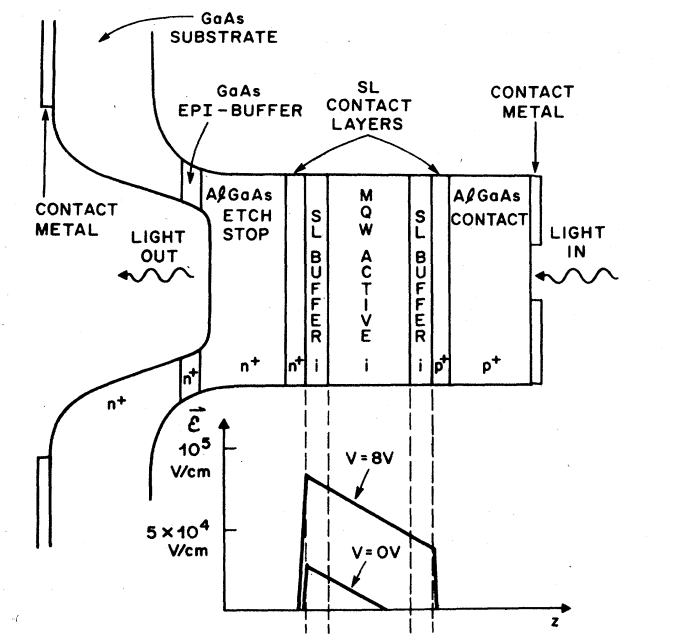
\includegraphics{images/Miller2-Figure2.png}
    }
    
    \caption{\label{fig:miller2-2}
        Схема измерений спектров поглощения в поперечном поле из работы \cite{miller1}.}
    \end {center}
    \end {figure}
    
    Если рисунок взят из какой-то статьи, книги или из интернета (из интернета нежелательно), то нужно обязательно в подписи сделать ссылку на соответствующий пункт в списке литературы.

    Ссылаемся на рисунок \ref{fig:miller2-2}.
    
    Ссылки на статьи: \cite{miller1}, \cite{miller2}, \cite{mohseni1}.

    Ссылка на российскую статью: \cite{skubachevskii1}.

    Ссылка на диссертацию:  \cite{pavlichenko1}

\subsection{Раздел 2}

% ============================================
% ГЛАВА 2
% ============================================
\pagebreak
\section{Теория и основные уравнения}

\subsection{Раздел 1}

Ненумерованная формула:

\begin{equation}
    \begin{pmatrix} \dot{\varphi}\\ \dot{\theta} \\ \dot{\psi} \end{pmatrix}
    = \begin{pmatrix}
        \cos(\theta)\cos(\psi) & -\sin(\psi) & 0 \\
        \cos(\theta)\sin(\psi) & \cos(\psi)  & 0 \\
        -\sin(\theta)         & 0         &  1
    \end{pmatrix}^{-1}
    \begin{pmatrix} \omega_x\\ \omega_y \\ \omega_z \end{pmatrix}. \nonumber
\end{equation}


\subsection{Раздел 2}

Нумерованные формулы:

\begin{equation}
\label{eq:1}
    \dot{\theta}=\frac{P-p_{1}\cos\left(\varphi_{1}-\theta\right)-p_{2}\cos\left(\varphi_{2}-\theta\right)}{\mu+\sin^{2}\left(\varphi_{1}-\theta\right)+\sin^{2}\left(\varphi_{2}-\theta\right)}
\end{equation}

\begin{equation}
    \dot{\varphi}_{1}=p_{1}-\dot{\theta}\cos(\phi_{1}-\theta)
\end{equation}

\begin{equation}
    \dot{\varphi}_{2}=p_{2}-\dot{\theta}\cos(\phi_{2}-\theta)
\end{equation}

Тест ссылки на формулу (\ref{eq:1}).

% ============================================
% ГЛАВА 3
% ============================================
\pagebreak
\section{Численные методы и алгоритмы}

\subsection{Раздел 1}

\subsection{Раздел 2}

% ============================================
% ГЛАВА 4
% ============================================
\pagebreak
\section{Программная реализация}

\begin{lstlisting}[language=rust,caption={Программная реализация метода Рунге-Кутты},label={listing-1}]
    // From the pendulum program
    fn runge_kutta(
        vars: &MyVec,
        pars: &Vec<f64>,
        rhs: &dyn Fn(&MyVec, &Vec<f64>) -> MyVec,
        dt: f64,
    ) -> MyVec {
        let rk_1 = rhs(vars, pars);
        let rk_2 = rhs(&vars.add(&rk_1.scale(dt / 2.0)), pars);
        let rk_3 = rhs(&vars.add(&rk_2.scale(dt / 2.0)), pars);
        let rk_4 = rhs(&vars.add(&rk_3.scale(dt)), pars);
    
        let vars_new = vars
            .add(&rk_1.scale(dt / 6.0))
            .add(&rk_2.scale(dt / 3.0))
            .add(&rk_3.scale(dt / 3.0))
            .add(&rk_4.scale(dt / 6.0));
        vars_new
    }
    \end{lstlisting}
    
    \begin{lstlisting}[language=C++,caption={Подпрограмма случайного блуждания на плоскости},label={listing-2}]
    std::random_device rd;
    std::mt19937 mt(rd());
    std::uniform_int_distribution<long> dist(1, 4);
    std::vector<long> xn(n0, 0);
    std::vector<long> yn(n0, 0);
    for (long jt = 0; jt < M; jt++)
    {
        for (long jn = 0; jn < n0; jn++)
        {
            switch (dist(mt))
            {
            case 1:
                xn[jn] ++;
                break;
            case 2:
                xn[jn] --;
                break;
            case 3:
                yn[jn] ++;
                break;
            case 4:
                yn[jn] --;
                break;
            }
        }
    }
    \end{lstlisting}

% ============================================
% ГЛАВА 5
% ============================================
\pagebreak
\section{Результаты и обсуждение}

Ниже тестируется очень большая таблица на несколько страниц

\begin{center}
    \begin{longtable}{|p{2cm}|p{3cm}|p{7cm}|p{3cm}|}
    \caption{Заголовок таблицы}\\
    \hline
    1 & 2 & 3 & 4\\ 
    \hline 
    2 & 2 & 3 & 4\\
    \hline
    3 & 2 & 3 & 4\\
    \hline
    4 & 2 & 3 & 4\\
    \hline
    5 & 2 & 3 & 4\\
    \hline
    6 & 2 & 3 & 4\\
    \hline
    7 & 2 & 3 & 4\\
    \hline
    8 & 2 & 3 & 4\\
    \hline
    9 & 2 & 3 & 4\\
    \hline
    10 & 2 & 3 & 4\\
    \hline
    1 & 2 & 3 & 4\\ 
    \hline 
    2 & 2 & 3 & 4\\
    \hline
    3 & 2 & 3 & 4\\
    \hline
    4 & 2 & 3 & 4\\
    \hline
    5 & 2 & 3 & 4\\
    \hline
    6 & 2 & 3 & 4\\
    \hline
    7 & 2 & 3 & 4\\
    \hline
    8 & 2 & 3 & 4\\
    \hline
    9 & 2 & 3 & 4\\
    \hline
    10 & 2 & 3 & 4\\
    \hline
    1 & 2 & 3 & 4\\ 
    \hline 
    2 & 2 & 3 & 4\\
    \hline
    3 & 2 & 3 & 4\\
    \hline
    4 & 2 & 3 & 4\\
    \hline
    5 & 2 & 3 & 4\\
    \hline
    6 & 2 & 3 & 4\\
    \hline
    7 & 2 & 3 & 4\\
    \hline
    8 & 2 & 3 & 4\\
    \hline
    9 & 2 & 3 & 4\\
    \hline
    10 & 2 & 3 & 4\\
    \hline
    
    
    \end{longtable}
\end{center}


А также тестируется счетчик таблиц, жирные и двойные линии.

\begin{center}
    \begin{longtable}{|p{2cm}||p{3cm}|p{7cm}|p{3cm}|}
    \caption{Заголовок таблицы номер 2}\\
    \hline
    1 & 2 & 3 & 4\\ 
    \hline
    2 & 2 & 3 & 4\\
    \hline
    3 & 2 & очень жирная ячейка \par с переносом & 4\\
    \hline
    4 & 2 & 3 & 4\\
    \hline
    5 & 2 & 3 & 4\\
    \hline
    6 & 2 & 3 & 4\\
    \hline
    7 & 2 & 3 & 4\\
    \hline
    8 & 2 & 3 & 4\\
    \hline
    9 & 2 & 3 & 4\\
    \hline
    10 & 2 & 3 & 4\\
    \hline
    
    
    \end{longtable}
\end{center}

Ссылаемся на Листинг \ref{listing-1} здесь.

% ============================================
%  ВЫВОДЫ И ЗАКЛЮЧЕНИЕ
% ============================================
\pagebreak
\specialsection{Выводы}
Структура файлов, которые можно редактировать:

\begin{itemize}
    \item \verb|main.tex| --- содержит основной текст;
    \item \verb|titlepage.tex| --- содержит титульный лист;
    \item \verb|literature.bib| --- содержит источники для списка литературы;
    \item \verb|code_highlight.tex| --- форматирование листингов (фрагментов кода).
\end{itemize}

Файл \verb|diploma.sty| очень важный, его трогать и особенно удалять не надо, там задаются различные стили документа.

\specialsection{Заключение}
Нужны ли отдельно и выводы, и заключение --- я не знаю. Разберёмся.

Список литературы ниже оформлен не по ГОСТу, но это легко исправить. Главное, что он организован, и можно ссылаться на каждый пункт по фамилии первого автора.

\textbf{Внимание!} 

Список литературы находится в отдельном файле \verb|literature.bib|, в который можно добавлять новые источники в любом порядке. Они будут сами располагаться как нужно, в порядке упоминания в тексте.

Если какой-то источник не процитирован в тексте, он в список литературы добавлен не будет.

Поэтому один и тот же файл с источниками можно использовать для нескольких документов.

\printbibliography

\end{document}